\chapter{Introduction}



\section{Overview}
In this chapter, the motivation and the background of this project will be presented and also the objectives will be fixed by the problems which have been found out to solve. This project will be able to fulfill the requirements of the teachers and students to create the utmost learning environment. In this project, I will build a dynamic website for both the teachers and students to practice their tasks according to their subjects. Here I propose a completely unique idea and a web-server throughout Bangladesh. My proposed system will be designed to ensure the learning and supervision of the students for their better development of studies. This website will help the students to complete their assignments on time, step-by-step processing and easier to understand the instructions given by the teachers. They will not need to use any other platforms like the classroom to submit all of their works.\\


\section{Background}
From the different researches, it is shown that the communication between students and teacher is being a critical factor day-by-day. Teachers are always responsible for ensuring a continuous learning environment for their students. According to statistical analysis of data from the Bangladeshi cities of Dhaka and Chattagram, online education results in negative pressure for both teaching and learning because of budgetary issues.\cite{rahman2021statistical}  Also, it is sometimes difficult to provide necessary resources, guidance and follow-up with the progress of the students. With the expansion of accredited university programs and broad internet access, online learning alternatives have grown rapidly. This online learning strategy promotes student growth, increases training flexibility, opens up new chances for group projects, and focuses on evaluation and feedback. However, universities are now working hard to be synchronous wherever possible by leveraging current information and communication technology (ICT). The maximum online platforms such as classroom, trello etc. are providing the following system.
\begin{figure}[H]
    \centering
    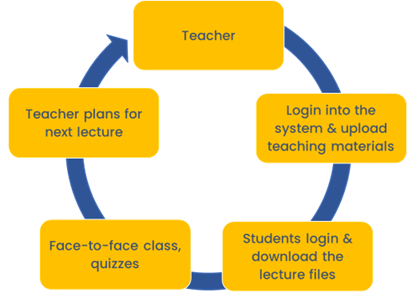
\includegraphics[scale=.9]{img/traditional.png}
    \caption{Traditional online enrollment system}
    \label{fig:System Architecture}
\end{figure}

The pandemic condition led to the transformation of formal education into online education with virtual classrooms that covered the fundamental needs for managing online education. IoT technology transforms classroom strategies in a useful way that makes it simpler to reduce time-consuming teacher and student practice concerns. In Bangladesh, though the online management system was maintained during the pandemic, after that it is being lost from the educational system. \\

As online education education is not practiced thoroughly in our country, results from online education are not always advantageous for the educational community since they raise a number of questions about the nature of online teaching and learning and raise public anxiety about the contentious subject of education. The current poll aims to illustrate the difficulties and opportunities faced by nations with less developed technology than those who have access to earlier contemporary technologies. \\

Despite not being in direct face-to-face contact with their instructors like in traditional classrooms, the majority of students have joined online classes with full enthusiasm, and informal surroundings have created a homely environment. However, internet disruptions and concerns about affordable bulk data availability remain significant challenges that need to be addressed to improve the education sector. It is essential to expand internet connectivity swiftly in distant locations and negotiate cost-effective data plans with cellular providers to assist students. These are the areas where national assistance is required to enhance the education system.\\

As the whole world and other universities of Bangladesh specially private universities are being virtualized, we also should build an online platform to keep pace with the modern world and to ensure effective and easier learning for the students.\\


\section{Problem Statement}
Under the current system, students are required to physically go and make appointments for final tasks without prior agreement on the subject with their teachers.
\begin{itemize}
    \item Under the current system, students are required to physically go and make appointments for final tasks without prior agreement on the subject with their teachers.

    
    \item Some researchers show that ongoing online platforms are not easier to access for sign-up.
    
    \item The results of the work can be beneficial to the governing bodies and owners of higher education institutions who are considering online education as a permanent fixture in the future.

    \item Some reliable systems are only available for the particular university and country.

    
    \item	Due to a shortage of resources, the online platforms in universities face numerous practical challenges.
    
    \item	There are many online platforms which can not provide not the security of data of the students and teachers. 

    
    \item Currently, either the main office staff or the lecturers themselves maintain the manual system, leading to an unnecessary increase in workload for the staff.

\end{itemize}


\section{Motivation}
In light of the decision of numerous knowledgeable students to pursue professional and academic opportunities at this university, it has expanded significantly over the years by adding new faculties and departments. However, this growth in enrollment has resulted in a declining relationship between professors and students throughout the university. Furthermore, the ratio of lecturers to students has decreased, making the current manual approach unsuitable for students who require guidance and wish to establish a better connection with their professors by meeting with supervisors.\\




\section{Objectives} 
This proposed system will serve the following objectives :
\begin{itemize}
    \item	To propose a novel model accompanied by easier methods, designed to function as a leading indicator and reduced complexity and time-consuming.


    \item	To develop this system by applying different user interfaces and also establishing a system according to the demands.

    \item	The proposed system will include detailed plans for hardware, operating systems, programming, and security considerations and  ensure the security issues for the users when they enter all of their personal data and information.



    % \item	The updated approach will try to address the shortcomings of the previous one while taking into account everyone from the supervisors to the pupils.


    % \item	The proposed system will include detailed plans for hardware, operating systems, programming, and security considerations.


    % \item	To ensure the security issues for the users when they enter all of their personal data and information.
\end{itemize}

% \newpage
\section{Research Outline}
The system is divided into four sections with different sub-sections and also demonstrated the required figures into it. In chapter II, there will be discussed related works in this area and which and how the model was used in those studies with detailed explanation. After that, I have briefed  the system model with the required figures to better understand in chapter III. For applying the models and building the system there will be needed the environment setup for programming and also the brief requirement analysis for this project which are entailed in the chapter IV. Then the implementation of the project will be shown and the result after applying different techniques are briefly explained in chapter IV. Finally, Chapter V will conclude the project by discussing potential areas for future work and improvements.






